%==============================================================================
%  Memory Tiering for Long-Context LLM Inference
%  Compile: pdflatex report.tex  (twice, for the ToC)
%==============================================================================
\documentclass[11pt,a4paper]{article}

\usepackage[T1]{fontenc}
\usepackage[utf8]{inputenc}
\IfFileExists{lmodern.sty}{\usepackage{lmodern}}{}
\usepackage[margin=2.5cm]{geometry}
\usepackage{booktabs}
\usepackage{longtable}
\usepackage{array}
\usepackage{xcolor}
\usepackage{tikz}
\usetikzlibrary{arrows.meta,positioning,calc,decorations.pathreplacing}
\usepackage{pgfplots}
\pgfplotsset{compat=1.17}
\usepackage{enumitem}
\usepackage{amsmath}
\usepackage{listings}
\lstset{
  backgroundcolor=\color{codebg}, frame=single, rulecolor=\color{codeframe},
  basicstyle=\ttfamily\scriptsize, breaklines=true, showstringspaces=false,
  columns=fullflexible, xleftmargin=5pt, xrightmargin=5pt,
  framexleftmargin=5pt, aboveskip=7pt, belowskip=7pt, tabsize=2,
  language=C++, commentstyle=\color{codecomment}\itshape,
}
\definecolor{codecomment}{RGB}{100,120,100}
\usepackage[hidelinks]{hyperref}

\definecolor{codebg}{RGB}{247,247,250}
\definecolor{codeframe}{RGB}{210,210,220}
\definecolor{noteblue}{RGB}{226,238,250}
\definecolor{warnamber}{RGB}{255,244,222}
\definecolor{oldgrey}{RGB}{238,238,240}
\definecolor{newgreen}{RGB}{230,245,232}
\definecolor{cCas}{RGB}{31,90,160}
\definecolor{cShb}{RGB}{230,140,40}
\definecolor{cSbs}{RGB}{60,150,80}
\definecolor{cHbf}{RGB}{200,50,50}

\newcommand{\callout}[3]{%
  \par\vspace{5pt}\noindent
  \begin{tikzpicture}
    \node[fill=#1,rounded corners=2pt,inner sep=8pt,
          text width=\dimexpr\linewidth-20pt\relax,align=left]
      {\textbf{#2}\ #3};
  \end{tikzpicture}\par\vspace{5pt}}
\newcommand{\note}[1]{\callout{noteblue}{Why.}{#1}}
\newcommand{\finding}[1]{\callout{newgreen}{Finding.}{#1}}
\newcommand{\warn}[1]{\callout{warnamber}{Caveat.}{#1}}
\newcommand{\code}[1]{\texttt{#1}}

\pgfplotsset{
  ap/.style={
    width=7.2cm, height=5.2cm,
    tick label style={font=\scriptsize}, label style={font=\scriptsize},
    title style={font=\small\bfseries},
    legend style={font=\scriptsize, draw=codeframe, fill=white, row sep=-1pt},
    grid=major, grid style={codeframe, very thin},
    every axis plot/.append style={thick, mark size=1.8pt},
  }}

\title{\textbf{Memory Tiering for Long-Context LLM Inference}\\[5pt]
  \large Evaluating H\textsuperscript{3}, comparing the arrangements it
  dismisses,\\ and a better one}
\author{}
\date{\today}

\begin{document}
\maketitle
\vspace{-2em}

\begin{abstract}
\noindent
Serving a large language model over a very long shared context is limited by
memory capacity, not by arithmetic. The H\textsuperscript{3} architecture
addresses this by adding a second, flash-based memory tier and placing
read-only data there. This report evaluates that proposal, then goes past it.
We compare H\textsuperscript{3}'s physical arrangement against three
alternatives it dismisses in a sentence, and find it wins --- but for a
different reason than claimed, and with a flash budget seventeen to sixty-seven
times larger than any of nine tested models can use. Reallocating that unused
flash to fast memory yields $1.75\times$ the concurrent requests at 21\% lower
power, identically across every model, because the mechanism is arithmetic
rather than model-specific. Finally we examine flash write endurance, and find
that the classic flash problem --- garbage collection --- is structurally
absent here, while a different one, wear concentration, decides device lifetime
by a factor of ten.
\end{abstract}

\tableofcontents
\vspace{1em}

%==============================================================================
\section{The problem: capacity, not arithmetic}
%==============================================================================

A GPU serving a language model must hold two things in memory at once:

\begin{itemize}[itemsep=2pt]
  \item \textbf{Model weights} --- fixed, read-only, and large. 405 GB for
        Llama-3.1-405B at 8-bit precision.
  \item \textbf{KV cache} --- per-request intermediate state, so that each new
        token need not re-derive everything the model has already seen. It grows
        with context length.
\end{itemize}

A B200 GPU offers 192 GB of HBM. The weights alone therefore span three GPUs
before a single request is served.

The situation becomes acute under \emph{cache-augmented generation}, where a
large document corpus is pre-processed once into a KV cache that every
subsequent query attends over. At one million tokens of shared context that
cache is roughly 540 GB; at ten million, 5.4 TB. Dozens of GPUs are then bought
purely as storage.

\subsection{Why this is a capacity problem and not a bandwidth one}

Decode is memory-bound: each generated token requires reading essentially all
the weights to perform a small amount of arithmetic. The standard remedy is
batching --- serve many requests at once so that one pass over the weights
amortises across all of them. Throughput is therefore roughly proportional to
batch size.

But batch size is set by \emph{leftover capacity}:
\[
  \text{batch} \;=\;
  \frac{\text{HBM} \;-\; \text{weights} \;-\; \text{shared cache} \;-\; \text{working set}}
       {\text{KV cache per request}}
\]

\note{Every gigabyte occupied by something that is not per-request state is a
gigabyte unavailable for concurrency. When the shared cache is 540 GB and the
GPU has 192 GB, the numerator is negative and the workload simply does not run.
This is the central quantity throughout this report: whatever increases the
numerator increases throughput almost linearly.}

\subsection{What H\textsuperscript{3} proposes}

High Bandwidth Flash (HBF) stacks NAND dies to reach HBM-comparable bandwidth
with roughly sixteen times the capacity, at four times the power per stack and
far worse write endurance.

H\textsuperscript{3}'s insight is that the two large consumers of capacity ---
weights and the shared cache --- are both \textbf{read-only}. Flash is poor at
writing and adequate at reading. So place them in flash, keep HBM for
per-request state, and the numerator above grows dramatically.

The proposal is sound. What this report examines is whether the specific
\emph{physical arrangement} and \emph{provisioning} chosen are the right ones.

%==============================================================================
\section{Method and validation}
%==============================================================================

We extended an analytical LLM inference simulator (LLMSimulator, SNU SCALE lab)
which models a single HBM tier only. Timing follows a roofline model per
operation,
\[
  t = \max\!\left(\frac{\text{FLOPs}}{\text{peak rate}},\;
                  \frac{\text{bytes}}{\text{bandwidth}}\right)
\]
so the entire cost model reduces to counting arithmetic and bytes and dividing
by peak rates. Introducing a second memory tier therefore means, concretely:
splitting the byte count between two bandwidths, and rewriting the capacity
budget that determines batch size.

\subsection{What was changed, and where}

Six concerns, roughly 900 lines. Paths are relative to \code{src/}, except
\code{test.cpp} and \code{validate\_config.h} which live in \code{eval/}.

\paragraph{1. A second memory tier.}
The simulator divided every operation's byte count by a single bandwidth. It now
splits that count across two tiers and takes whichever is slower --- or, where
both tiers share one link to the GPU, charges their sum against that link.

\begin{center}\small
\begin{tabular}{@{}p{5.0cm}p{9.3cm}@{}}
\toprule
\code{hardware\_config.h} & \code{B200\_H3} preset: \code{hbf\_capacity},
  \code{hbf\_bandwidth}, \code{num\_hbf\_cube},
  \code{shared\_link\_bandwidth}, \code{link\_topology} \\
\code{layer\_impl.cpp} & \code{h3MemoryDuration()} --- the two-tier timing
  helper every operation now calls \\
\code{tensor.cpp} & \code{in\_hbf} set at construction from the tensor's tag:
  \code{weight} and \code{cache\_shared} to flash, all else to HBM \\
\code{linear\_impl.cpp} & weight bytes routed through the two-tier path \\
\bottomrule
\end{tabular}
\end{center}

\begin{lstlisting}[caption={\code{layer\_impl.cpp} --- the whole two-tier cost model},captionpos=b]
time_ns h3MemoryDuration(SystemConfig config, hw_metric hbm_bytes,
                         hw_metric hbf_bytes) {
  time_ns hbm_duration = hbm_bytes / config.memory_bandwidth * 1e9;
  if (!config.use_hbf || hbf_bytes <= 0) return hbm_duration;

  hw_metric hbf_bw = config.hbf_bandwidth * config.hbf_bandwidth_scale;
  time_ns hbf_duration = hbf_bytes / hbf_bw * 1e9;

  // Pooled link: both tiers cross one connection, so transfers serialize.
  // The flash media bandwidth remains a second, independent cap.
  if ((config.link_topology == "cascaded" ||
       config.link_topology == "shared_base") &&
      config.shared_link_bandwidth > 0) {
    time_ns link = (hbm_bytes + hbf_bytes)
                 / config.shared_link_bandwidth * 1e9;
    return std::max(link, hbf_duration);
  }
  // Independent paths: transfers overlap, slower tier sets the duration.
  return std::max(hbm_duration, hbf_duration);
}
\end{lstlisting}

\begin{lstlisting}[caption={\code{tensor.cpp} --- placement follows the tag, so no call site decides},captionpos=b]
if (device != nullptr && device->config.use_hbf &&
    (tag == "weight" || tag == "cache_shared")) {
  in_hbf = true;   // read-only data -> flash; everything else stays in HBM
}
\end{lstlisting}

\paragraph{2. A genuinely shared read-only cache.}
The original created one cache per request per attention head --- correct for
private conversations, but it would have counted a shared corpus once per user.
There is now a single shared-cache tensor per layer, sized independently of
batch, with its length derived from the workload rather than configured by hand.

\begin{center}\small
\begin{tabular}{@{}p{5.0cm}p{9.3cm}@{}}
\toprule
\code{model\_config.h} & \code{shared\_kv\_cache\_len},
  \code{cag\_amortize\_shared\_compute} \\
\code{test.cpp} & derives shared length as
  $\text{context window} - \text{ISL} - \text{OSL}$ \\
\code{attention.cpp} & creates one \code{cache\_shared} tensor per layer \\
\code{module.cpp} & fourth size category, so shared cache is budgeted apart
  from private KV \\
\code{attention\_gen\_impl.cpp} & shared-span attention cost; amortisation
  charges that span once per batch rather than once per request \\
\bottomrule
\end{tabular}
\end{center}

\begin{lstlisting}[caption={\code{attention.cpp} --- one shared tensor per layer, sized independently of batch},captionpos=b]
if (device->model_config.shared_kv_cache_len > 0) {
  // context_parallel_degree > 1 splits the shared cache across the devices
  // that jointly own this KV head -- each holds a 1/cp_dg slice.
  int cp_dg = device->model_config.context_parallel_degree;
  int shared_len_local = device->model_config.shared_kv_cache_len / cp_dg;
  std::vector<int> shared_shape = {shared_len_local, head_dim * num_kv_heads};
  k_cache_shared = Tensor::Create("k_cache_shared", shared_shape,
                                  "cache_shared", device, kv_precision);
  v_cache_shared = Tensor::Create("v_cache_shared", shared_shape,
                                  "cache_shared", device, kv_precision);
}
\end{lstlisting}

\begin{lstlisting}[caption={\code{test.cpp} --- shared length derived from the workload, not configured},captionpos=b]
// Whatever the context window holds beyond one request's own input and
// output is the shared pre-computed cache every request attends over.
model_config.shared_kv_cache_len = context_window - input_len - output_len;
\end{lstlisting}

\paragraph{3. The capacity budget --- where the benefit appears.}
This single function decides batch size, and therefore throughput. Flash now
absorbs weights and shared cache, leaving HBM free for per-request state.

\begin{center}\small
\begin{tabular}{@{}p{5.0cm}p{9.3cm}@{}}
\toprule
\code{cluster.cpp} & \code{checkH3MemorySize()}: flash holds weights $+$
  shared cache (checked against flash capacity separately); free HBM is
  capacity minus working set only \\
\bottomrule
\end{tabular}
\end{center}

\begin{lstlisting}[caption={\code{cluster.cpp} --- the two budgets. \code{size\_vector} is [act, weight, cache, cache\_shared]},captionpos=b]
// Flash: weights + shared cache. Both read-only, both batch-independent.
double hbf_size = size_vector.at(1) + size_vector.at(3);
if (hbf_size > config.hbf_capacity)
  fail("weights + shared KV cache exceed HBF capacity");

// HBM: activations + private KV only. Note what is ABSENT compared with
// checkMemorySize() -- weights and shared cache are not subtracted, which
// is exactly what frees capacity for a larger batch.
double hbm_size = (size_vector.at(0) / num_layers) + size_vector.at(2);

hw_metric avail = config.memory_capacity * (1.0 - config.hbm_reserve_fraction)
                - (size_vector.at(0) / num_layers);
int max_batch_size = (int)(avail / kv_cache_size_per_seq) * dp_degree;
\end{lstlisting}

\warn{The HBM-only baseline in \code{checkMemorySize()} needed correcting too.
Without flash the shared cache has nowhere else to go, so it must be charged to
HBM. Omitting that would have understated the baseline's own footprint and
flattered every comparison against it.}

\paragraph{4. Reaching 32 GPUs.}
Attention work was divided by assigning each device a whole KV head, capping
parallelism at eight for Llama-3.1-405B. The ten-million-token configuration
needs thirty-two. A second axis now lets groups of devices share a head and
split the shared cache by length, with a combine step afterwards.

\begin{center}\small
\begin{tabular}{@{}p{5.0cm}p{9.3cm}@{}}
\toprule
\code{parallel.cpp} & \code{context\_parallel\_degree}; combine step reuses the
  existing all-reduce cost model \\
\code{communication.cpp} & \code{AllReduce::forward} derives each rank's node
  as \code{rank / num\_device} and charges the scale-out fabric when a group
  spans nodes \\
\bottomrule
\end{tabular}
\end{center}

\begin{lstlisting}[caption={\code{parallel.cpp} --- a second sharding axis lifts the KV-head ceiling},captionpos=b]
// parallel_num (= ne_tp_dg) may now exceed num_kv_heads. head_tp_dg is the
// degree for whole-KV-head sharding; the remaining cp_dg devices inside each
// head's group split the shared cache BY LENGTH instead.
int cp_dg = device->model_config.context_parallel_degree;
assertTrue(parallel_num % cp_dg == 0,
           "ne_tp_dg must be divisible by context_parallel_degree");
int head_tp_dg = parallel_num / cp_dg;
\end{lstlisting}

\begin{lstlisting}[caption={\code{communication.cpp} --- which fabric a collective actually crosses},captionpos=b]
for (int rank : device_list) spanned_nodes.insert(rank / device_per_node);
const int num_span_node   = std::max(1, (int)spanned_nodes.size());
const int group_per_node  = std::max(1, num_group_device / num_span_node);

if (num_span_node == 1) {
  // One NVLink domain: unchanged.
} else if (device->config.allreduce_hierarchical) {
  // Reduce-scatter inside each node, ring across nodes, all-gather inside.
  // Only size/group_per_node ever crosses the slow scale-out fabric.
} else {
  // Flat ring: every step is gated by the inter-node link.
}
\end{lstlisting}

\warn{The collective previously charged NVLink bandwidth to every group,
including ones spanning four physical servers. This is a defect in the base
simulator rather than a modelling choice: the paper explicitly states that its
ten-million-token runs cross a scale-out fabric, which is roughly nine times
slower.}

\paragraph{5. Configurable physical arrangements.}
So that the four layouts of Section~3 and the mixed-die designs of Section~5 are
configuration rather than code.

\begin{center}\small
\begin{tabular}{@{}p{5.0cm}p{9.3cm}@{}}
\toprule
\code{test.cpp} & \code{architecture} $\in$ \{\code{cascaded},
  \code{side\_by\_side}, \code{shared\_base}, \code{hbf\_only}\} with
  \code{hbm\_sites}, \code{hbf\_sites}, \code{hbm\_dies\_per\_site},
  \code{hbf\_dies\_per\_site} against a \code{shoreline\_slots} budget.
  Derives per-tier capacity and bandwidth, and whether the link is pooled \\
\code{model\_config.h} & \code{kv\_cache\_precision\_byte}, independent of
  weight precision \\
\code{hardware\_config.h} & \code{gpu\_tdp}, \code{hbm\_tdp\_per\_cube},
  \code{hbf\_tdp\_per\_cube}; per-device total
  $680 + 40\,n_{\text{hbm}} + 160\,n_{\text{hbf}}$ watts \\
\bottomrule
\end{tabular}
\end{center}

\paragraph{6. The write path.}
Flash sees no writes under H\textsuperscript{3}'s placement, so studying
endurance requires a mechanism that produces them: admit beyond the HBM ceiling
and let the excess private KV spill.

\begin{center}\small
\begin{tabular}{@{}p{5.0cm}p{9.3cm}@{}}
\toprule
\code{cluster.cpp} & \code{hbm\_oversubscribe\_fraction}: admit past the HBM
  ceiling so the excess must spill \\
\code{transient\_kv\_manager.cpp} & per-request residency, LRU eviction,
  migration and append accounting \\
\code{hbf\_flash.h} & DRAM write-combining buffer; block-level flash with
  greedy collection and an erase histogram. Makes write amplification a
  measured output rather than a constant \\
\bottomrule
\end{tabular}
\end{center}

\begin{lstlisting}[caption={\code{cluster.cpp} --- admitting past the HBM ceiling forces a spill},captionpos=b]
int hbm_resident_batch = (int)(avail / kv_cache_size_per_seq) * dp_degree - 1;
int max_batch_size = hbm_resident_batch + 1;
if (config.hbm_oversubscribe_fraction > 0.0) {
  max_batch_size = (int)(hbm_resident_batch *
                         (1.0 + config.hbm_oversubscribe_fraction)) + 1;
  // Everything above hbm_resident_batch has no HBM to live in and must be
  // migrated to flash by TransientKvManager.
}
\end{lstlisting}

The residency model is driven once per decode step from the live batch, which is
the only point where the post-cap request count and each request's actual length
are both known. Requests absent from a call have finished and are released.

\begin{lstlisting}[caption={\code{cluster.cpp} --- driving residency from the live batch each step},captionpos=b]
auto metadata = scheduler->setMetadata();
if (config.use_hbf) {
  for (int d = 0; d < total_dev; d++) {
    auto seqs = metadata.at(...)->get_seq();
    std::vector<int> ids; std::vector<long> lens;
    for (size_t i = 0; i < seqs.size(); i++) {
      ids.push_back((int)i);
      lens.push_back((long)seqs.at(i)->current_len);   // ACTUAL length
    }
    get_device(d)->kv_manager().sync_batch(ids, lens);
  }
}
\end{lstlisting}

\code{sync\_batch} decides everything. A request's footprint is its live length
times a per-token constant; when the total exceeds the HBM budget, the
least-recently-touched resident request is evicted to flash.

\begin{lstlisting}[caption={\code{transient\_kv\_manager.cpp} --- the two write populations arise here},captionpos=b]
for each request i in the batch:
  long want = seq_lens[i] * kv_bytes_per_token_;     // 2 * L * kvh * dim * prec
  if (not tracked)      { admit;  hbm_used_ += want; }
  else if (in flash)    {
      // POPULATION 2 -- APPEND. This request already lives in flash, so its
      // new tokens are a small write: 512 B per layer per step. This is the
      // population the write-combining buffer exists for.
      long grew = want - rec.bytes;
      long flushed = wbuf_.append(id, grew);
      if (flushed) phys = flash_.write(blocks * threshold, flushed, id);
  }
  else                  { hbm_used_ += (want - rec.bytes); }

make_room_if_needed();   // evict LRU while hbm_used_ > budget

// POPULATION 1 -- MIGRATION. A whole cache moves at once: ~62 MB, i.e. 62
// contiguous blocks. Already block-aligned, so it bypasses the buffer.
void spill_to_hbf(int id) {
  rec.in_hbf = true;
  hbm_used_ -= rec.bytes;
  long physical = flash_.write(rec.bytes, id);
}
\end{lstlisting}

\begin{lstlisting}[caption={\code{hbf\_flash.h} --- combining the small appends, which is where amplification comes from},captionpos=b]
// Appends arrive per (layer, request) at 512 B against a 4096 B page, so
// unbuffered amplification is 8x. Accumulate until a fraction of an erase
// block has gathered, then write once. Waste at flush IS the amplification.
long append(int stream, long bytes) {
  fill_[s] += bytes;
  long flushed = 0;
  while (fill_[s] >= threshold_bytes_) {
    flushed  += block_bytes_;                       // a whole block consumed
    fill_[s] -= threshold_bytes_;
    wasted_  += block_bytes_ - threshold_bytes_;
  }
  return flushed;
}
\end{lstlisting}

\note{The buffer costs no extra traffic. Appended tokens are \emph{already in
HBM} --- a spilled request still generates its new state there, and only its
older cache sits in flash. Buffering does not add a copy; it defers a flush. The
sole cost is that a spilled request does not fully vacate HBM, which at
per-request granularity is 0.6\% of the KV budget.}

Flash itself is modelled at block granularity, so amplification and erase counts
are measured rather than assumed. The distinction that matters is
\code{logical\_bytes} versus \code{raw\_bytes}: the buffer hands over whole
blocks, and recording those as host writes would make amplification invisible.

\begin{lstlisting}[caption={\code{hbf\_flash.h} --- block model, greedy collection, and why the two byte counts differ},captionpos=b]
struct Block { int valid_pages, written_pages; uint64_t erase_count;
               int owner_seq; };   // owner_seq enables death correlation

// logical_bytes = what the workload produced.
// raw_bytes     = whole blocks the buffer hands over, incl. flush waste.
long write(long logical_bytes, long raw_bytes, int seq_id) {
  stats_.host_write_bytes += logical_bytes;          // NOT raw_bytes
  long physical = ceil(raw_bytes / page_bytes_) * page_bytes_;
  // ... fill the open block for this request; allocate a fresh one if full
  stats_.physical_write_bytes += physical;
  return physical + maybe_collect();
}

// A finished request invalidates every page it owns. With per-request block
// allocation those are WHOLE blocks, so they become erasable with zero
// copying -- the death-correlation property of KV cache.
void invalidate_sequence(int seq_id) {
  for each block b with owner_[b] == seq_id: valid_[b] = 0;
}

// Greedy collection: victim = fewest valid pages. Survivors are relocated,
// and that relocation is the amplification a collector adds.
long collect() {
  pick block with min valid_pages (excluding open blocks);
  stats_.gc_copy_bytes       += valid_[victim] * page_bytes_;
  stats_.physical_write_bytes += valid_[victim] * page_bytes_;
  erases_[victim]++;  written_[victim] = valid_[victim] = 0;
  free_.push_back(victim);
}

double waf() const {                 // the measured output
  return double(physical_write_bytes) / host_write_bytes;
}
\end{lstlisting}

\warn{Endurance is limited by the \emph{worst} block, not the mean, so
\code{erase\_histogram()} reports mean, p99 and maximum, and
\code{projected\_life\_years()} is computed from the maximum. A mean erase count
would flatter the result substantially, because the static region never wears at
all (Section~7.7).}

Every knob above is a YAML key under \code{system:} or \code{simulation:}.
\code{validate\_config.h} rejects any key the code does not read and warns when
one that materially changes results is absent, so a configuration cannot
silently mean something other than it appears to.

Before drawing any new conclusions we reproduced the original results.

\begin{table}[h]
\centering\small
\begin{tabular}{@{}lccl@{}}
\toprule
\textbf{1 M context, 8 GPUs} & \textbf{Ours} & \textbf{Published} & \\
\midrule
Batch size ratio    & 2.71$\times$  & 2.6$\times$   & calibration target \\
Throughput ratio    & 1.261$\times$ & 1.25$\times$  & \emph{not} a target; $+0.9\%$ \\
Throughput per watt & 0.553$\times$ & 0.548$\times$ & \emph{not} a target; $+0.9\%$ \\
\bottomrule
\end{tabular}
\end{table}

Only the batch ratio was used for calibration; the other two agree within 1\%
without being fitted.

\subsection{An arithmetic check on the paper's headline number}

The paper reports its throughput and its throughput-per-power in different
subsections, and never states the power ratio connecting them. That ratio is
derivable from three constants it does state, which makes the two results a
consistency check on each other.

\textbf{Inputs}, all from the paper (Sections IV-A.3 and IV-B.3): GPU
\textbf{680 W} --- explicitly ``without HBM or HBF''; HBM3E \textbf{40 W per
cube}; HBF \textbf{160 W per cube}; eight cubes of each per GPU.

\textbf{Step 1 --- power per GPU.}
\begin{align*}
  \text{HBM-only} &= 680 + (8 \times 40) = 1000\ \text{W} \\
  \text{H}^3      &= 680 + (8 \times 40) + (8 \times 160) = 2280\ \text{W} \\[2pt]
  \text{power ratio} &= 2280 / 1000 = 2.28
\end{align*}

\textbf{Step 2 --- close the loop.} Throughput-per-power \emph{is} throughput
divided by power, so the paper's two independently-reported ten-million-token
figures must be consistent with that ratio:
\[
  \frac{\text{throughput ratio } 6.14}{\text{power ratio } 2.28}
  \;=\; \mathbf{2.693}
  \qquad\text{against the published } 2.69\times.
\]

\finding{Agreement to three digits. This confirms three things at once: the TDP
constants are what we read them to be, the cube counts are eight and eight, and
the paper's throughput and efficiency figures come from the same run rather than
different configurations.}

The same arithmetic at one million tokens is a \emph{prediction} rather than a
confirmation, because the paper gives no numeric efficiency figure there --- only
a chart. Its own arithmetic implies $1.25 / 2.28 = 0.548$, and our simulator
independently produced $0.553$: within 1\%, and never calibrated against it.

\warn{This validates the \emph{power} model only. It says nothing about whether
the timing model is right --- that is what the one-million-token throughput
ratio (1.261 against 1.25) tests, and that one is a simulation result rather
than arithmetic.}

At ten million tokens the reported throughput gain falls inside a bracket set by
an ambiguity in the paper's own description --- it specifies ``ring all-reduce''
without saying whether the ring is flat or hierarchical, and across four
physical servers those differ substantially. Our flat-ring reading gives
$3.60\times$ and our hierarchical reading $7.21\times$, against the published
$6.14\times$.

\note{One consequence of the replication is worth stating because it looks like
a failure and is not. At one million tokens, throughput-per-watt is
\emph{below} unity --- H\textsuperscript{3} loses. The paper's own arithmetic
implies 0.548, and its headline ``up to 2.69$\times$'' refers only to the ten
million case. Flash costs four times the power of HBM per stack, so the capacity
gain must be large before it pays for itself. Reproducing the regime where the
idea does \emph{not} work is part of establishing that the model behaves.}

%==============================================================================
\section{Four physical arrangements}
%==============================================================================

H\textsuperscript{3} chains flash \emph{behind} the HBM stacks and argues in one
sentence that placing them side by side would waste GPU edge area. It never
tests this. With a working two-tier model the question is answerable.

A GPU edge accommodates a fixed number of memory sites --- eight on the B200,
each carrying about 1 TB/s. A site holds a stack of eight dies; an HBM die is
3 GB, a flash die 48 GB. The arrangements differ only in how those eight sites
are spent.

\begin{figure}[h]
\centering
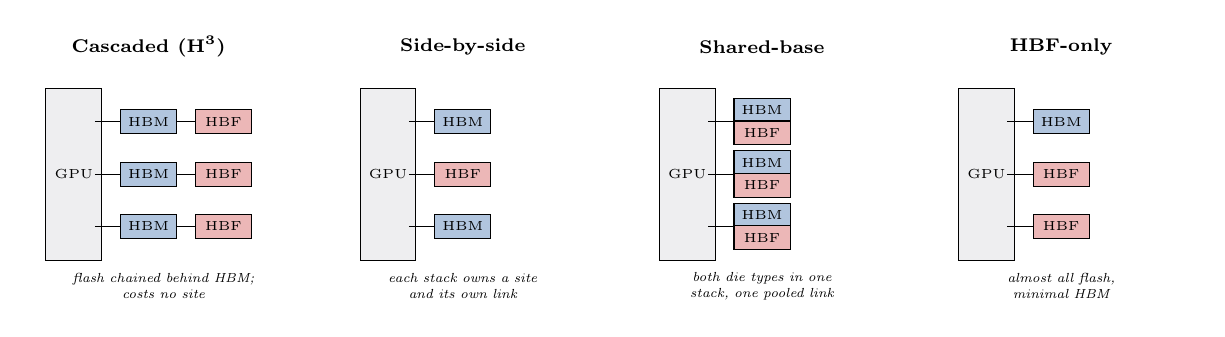
\begin{tikzpicture}[
  gpu/.style={draw, fill=oldgrey, minimum width=0.55cm, minimum height=2.3cm, font=\tiny},
  hbm/.style={draw, fill=cCas!35, minimum width=0.75cm, minimum height=0.32cm, font=\tiny, inner sep=1pt},
  hbf/.style={draw, fill=cHbf!35, minimum width=0.75cm, minimum height=0.32cm, font=\tiny, inner sep=1pt},
  hdg/.style={font=\scriptsize\bfseries},
  sub/.style={font=\tiny\itshape, text width=3.4cm, align=center},
  scale=0.95, transform shape]
\begin{scope}[xshift=0cm]
  \node[hdg] at (1.0,1.7) {Cascaded (H\textsuperscript{3})};
  \node[gpu] at (0,0) {GPU};
  \foreach \y in {0.7,0,-0.7}{
    \node[hbm] at (1.0,\y) {HBM}; \node[hbf] at (2.0,\y) {HBF};
    \draw[very thin] (0.28,\y) -- (0.62,\y); \draw[very thin] (1.38,\y) -- (1.62,\y);}
  \node[sub] at (1.2,-1.5) {flash chained behind HBM;\\costs no site};
\end{scope}
\begin{scope}[xshift=4.2cm]
  \node[hdg] at (1.0,1.7) {Side-by-side};
  \node[gpu] at (0,0) {GPU};
  \node[hbm] at (1.0,0.7) {HBM}; \node[hbf] at (1.0,0) {HBF}; \node[hbm] at (1.0,-0.7) {HBM};
  \foreach \y in {0.7,0,-0.7}{\draw[very thin] (0.28,\y) -- (0.62,\y);}
  \node[sub] at (1.0,-1.5) {each stack owns a site\\and its own link};
\end{scope}
\begin{scope}[xshift=8.2cm]
  \node[hdg] at (1.0,1.7) {Shared-base};
  \node[gpu] at (0,0) {GPU};
  \foreach \y/\yy in {0.85/0.55, 0.15/-0.15, -0.55/-0.85}{
    \node[hbm] at (1.0,\y) {HBM}; \node[hbf] at (1.0,\yy) {HBF};
    \draw[very thin] (0.28,{(\y+\yy)/2}) -- (0.62,{(\y+\yy)/2});}
  \node[sub] at (1.0,-1.5) {both die types in one\\stack, one pooled link};
\end{scope}
\begin{scope}[xshift=12.2cm]
  \node[hdg] at (1.0,1.7) {HBF-only};
  \node[gpu] at (0,0) {GPU};
  \node[hbm] at (1.0,0.7) {HBM}; \node[hbf] at (1.0,0) {HBF}; \node[hbf] at (1.0,-0.7) {HBF};
  \foreach \y in {0.7,0,-0.7}{\draw[very thin] (0.28,\y) -- (0.62,\y);}
  \node[sub] at (1.0,-1.5) {almost all flash,\\minimal HBM};
\end{scope}
\end{tikzpicture}
\caption{Only the cascaded arrangement adds flash without surrendering an HBM
site.}
\end{figure}

\begin{table}[h]
\centering\small
\begin{tabular}{@{}lccccc@{}}
\toprule
\textbf{Arrangement} & \textbf{Sites} & \textbf{HBM} & \textbf{Flash} & \textbf{Link} & \textbf{Power} \\
\midrule
Cascaded (H\textsuperscript{3}) & 8   & 192 GB & 3072 GB & pooled      & 2280 W \\
Shared-base                     & 8   & 96 GB  & 1536 GB & pooled      & 1480 W \\
Side-by-side                    & 4+4 & 96 GB  & 1536 GB & partitioned & 1480 W \\
HBF-only                        & 1+7 & 24 GB  & 2688 GB & partitioned & 1840 W \\
\bottomrule
\end{tabular}
\end{table}

Cascaded is fastest at every context length. The interesting question is why.

\subsection{Capacity dominates wiring, and by roughly two to one}

Cascaded has both more HBM \emph{and} more flash than its rivals, so a raw
comparison confounds two effects. Running every arrangement at a
\emph{pinned} request count removes capacity from the comparison and leaves
only the wiring:

\begin{table}[h]
\centering\small
\begin{tabular}{@{}lrrrr@{}}
\toprule
\textbf{Pinned batch} & \textbf{Cascaded} & \textbf{Shared-base} & \textbf{Side-by-side} & \textbf{Cascaded gain} \\
\midrule
175 & 433.7 & 281.9 & 273.5 & $+53.8\%$ \\
400 & 649.7 & 484.1 & 459.8 & $+34.2\%$ \\
725 & 779.0 & 640.3 & 598.3 & $+21.7\%$ \\
\bottomrule
\end{tabular}
\caption{Tokens per second at equal request count. Any difference here is
attributable to memory arrangement alone.}
\end{table}

At its own maximum batch, cascaded beats shared-base by $2.45\times$. Decomposed:

\[
  \underbrace{1.22\times}_{\text{wiring}} \;\times\;
  \underbrace{2.01\times}_{\text{capacity (1457 vs 724 requests)}}
  \;=\; 2.45\times
\]

\finding{Cascaded wins because it \textbf{protects HBM sites}, not because it
supplies flash bandwidth. Capacity contributes roughly twice what wiring does. A
confirming experiment: re-running cascaded with only half its flash --- matching
shared-base exactly on the flash tier --- still left it 23\% ahead at ten
million tokens.}

The wiring advantage also \emph{shrinks} as batch grows, from 54\% to 22\%. At
small batch, flash traffic (weights plus shared cache) dominates and cascaded's
full bandwidth to flash matters greatly. As batch grows, per-request KV traffic
on HBM takes over and the flash advantage dilutes.

\subsection{Pooling a link beats partitioning it, in proportion to the mix}

Shared-base and side-by-side can be built at matched capacity, matched aggregate
bandwidth and matched power. Only the wiring differs: one pools a single link,
the other fixes a split. Sweeping the HBM/flash ratio across seven matched pairs:

\begin{figure}[h]
\centering
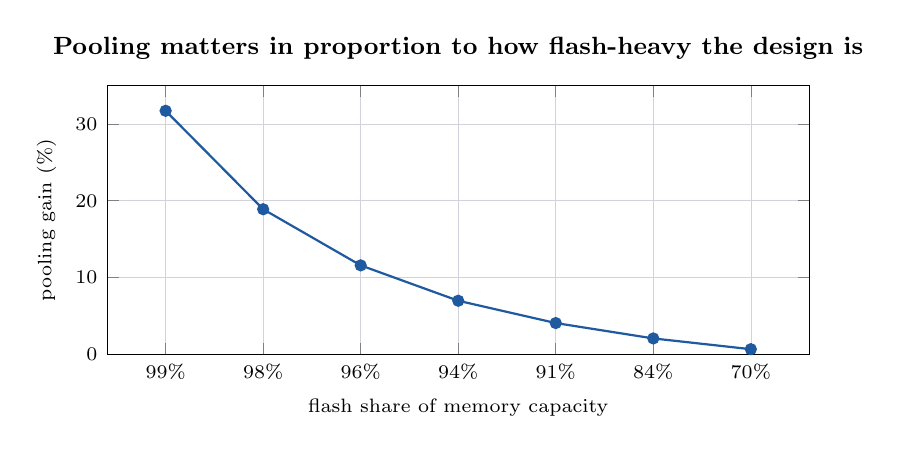
\begin{tikzpicture}
\begin{axis}[ap, width=10.5cm, height=5cm,
  xlabel={flash share of memory capacity}, ylabel={pooling gain (\%)},
  title={Pooling matters in proportion to how flash-heavy the design is},
  xtick={0,1,2,3,4,5,6},
  xticklabels={99\%,98\%,96\%,94\%,91\%,84\%,70\%}, ymin=0, ymax=35]
\addplot[cCas, mark=*] coordinates {(0,31.7)(1,18.9)(2,11.6)(3,7.0)(4,4.1)(5,2.1)(6,0.7)};
\end{axis}
\end{tikzpicture}
\caption{From $+0.7\%$ to $+31.7\%$, monotonic in flash share.}
\end{figure}

\note{A fixed split cannot lend bandwidth. When one tier is busy and the other
idle, the idle half is wasted. Pooling lets whichever tier needs the bandwidth
consume all of it. The more of the machine that sits behind the flash half of a
fixed split, the more bandwidth goes unlent --- which is why the gain scales with
flash share. This is a design rule rather than a single measurement: pool the
link in proportion to how flash-heavy the design is.}

\warn{Our shared-link model charges nothing for pooling, so pooling cannot lose
in this simulator. The \emph{direction} of this result is assumed; only its
magnitude is measured.}

\subsection{All-flash fails on capacity, not on speed}

HBF-only is worst on raw throughput, but the reason matters. At a
\emph{matched} request count of 175 it actually \emph{beats} both shared-base
and side-by-side (305.7 against 281.9 and 273.5) --- its 7 TB/s of flash
bandwidth is genuinely useful.

\finding{HBF-only fails because 24 GB of HBM caps it at 174 concurrent requests
against cascaded's 1457. It is \textbf{capacity-limited, not slow}. ``All-flash
is too slow'' would be the wrong lesson; ``all-flash starves concurrency'' is
the right one.}

%==============================================================================
\section{H\textsuperscript{3} over-provisions flash by more than an order of magnitude}
%==============================================================================

Flash holds exactly two things: weights and the shared cache. Both are
computable in closed form from a model definition, with no simulation.

\begin{table}[h]
\centering\small
\begin{tabular}{@{}lrrr@{}}
\toprule
\textbf{Model} & \textbf{Weights} & \textbf{KV / token} & \textbf{Flash needed / device} \\
\midrule
mixtral          &  93 GB & 131 KB &  45.9 GB \\
llama4\_scout    & 216 GB & 197 KB &  71.2 GB \\
llama4\_maverick & 801 GB & 197 KB &  89.5 GB \\
grok1            & 633 GB & 262 KB & 105.7 GB \\
openMoE          &  66 GB & 393 KB & 130.9 GB \\
llama7bMoE       &  13 GB & 524 KB & 172.2 GB \\
glam             & 288 GB & 524 KB & 180.8 GB \\
llama3\_405B     & 406 GB & 516 KB & 181.8 GB \\
\midrule
\textbf{deepseekV3} & 709 GB & \textbf{3932 KB} & \textbf{1310.7 GB} \\
\bottomrule
\end{tabular}
\caption{Flash residency at ten million tokens, per device at 32-way tensor
parallelism.}
\end{table}

\finding{Eight of nine models need under 182 GB. One flash die per site provides
384 GB. H\textsuperscript{3} ships \textbf{eight} dies --- 3072 GB --- between
17 and 67 times more than those eight models can use. Only DeepSeek-V3 needs
more, because multi-head latent attention at 128 KV heads gives it a per-token
footprint 7.6 times Llama's.}

\note{This reframes the provisioning. H\textsuperscript{3}'s eight dies are not
arbitrary --- they are correctly sized for a latent-attention model with many KV
heads. For every other model in the set they are near-idle silicon drawing
160 W per stack. The right conclusion is not ``H\textsuperscript{3} has too much
flash'' but ``flash depth should be configurable, and is set by an outlier
rather than by the workload in general.'' The paper does not ask this question.}

%==============================================================================
\section{A better arrangement: mixed dies in the chained stack}
%==============================================================================

All four arrangements above treat a chained flash stack as \emph{entirely}
flash. If that capacity is unused, the dies behind it can be HBM instead. Keep
the front stack at eight HBM dies and make the chained stack a mixture.

The site link is unchanged, so this costs nothing in wiring --- it simply
reallocates silicon within the chain.

\begin{table}[h]
\centering\small
\begin{tabular}{@{}lrrrrrr@{}}
\toprule
\textbf{Design} & \textbf{HBM} & \textbf{Flash} & \textbf{Requests} & \textbf{tokens/s} & \textbf{tokens/s/W} & \textbf{Power} \\
\midrule
8H8F (H\textsuperscript{3}) & 192 GB & 3072 GB & 1457 & \textbf{8881} & 0.1218 & 2280 W \\
10H6F        & 240 GB & 2304 GB & 1824 & 8839 & 0.1354 & 2040 W \\
12H4F        & 288 GB & 1536 GB & 2191 & 8579 & 0.1489 & 1800 W \\
14H2F        & 336 GB & 768 GB  & 2557 & 7721 & \textbf{0.1547} & 1560 W \\
15H1F        & 360 GB & 384 GB  & 2741 & 6380 & 0.1384 & 1440 W \\
\bottomrule
\end{tabular}
\caption{Cascaded, eight sites, varying the die split inside the chained stack.
Llama-3.1-405B at ten million tokens.}
\end{table}

\begin{figure}[h]
\centering
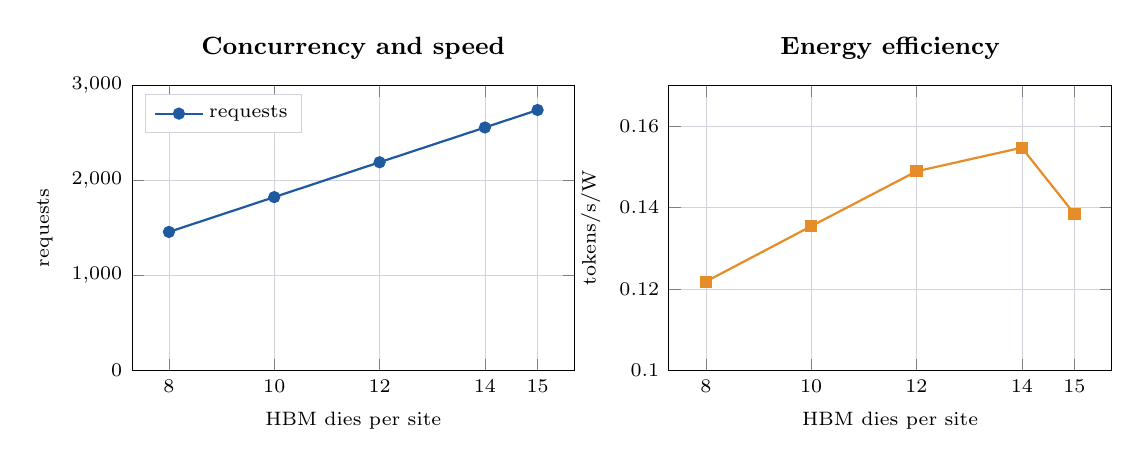
\begin{tikzpicture}
\begin{axis}[ap, name=a, title={Concurrency and speed},
  xlabel={HBM dies per site}, ylabel={requests}, xtick={8,10,12,14,15},
  ymin=0, ymax=3000, scaled y ticks=false,
  legend style={at={(0.03,0.97)}, anchor=north west}]
\addplot[cCas,mark=*] coordinates {(8,1457)(10,1824)(12,2191)(14,2557)(15,2741)};
\addlegendentry{requests}
\end{axis}
\begin{axis}[ap, at={(a.east)}, xshift=1.2cm, anchor=west,
  title={Energy efficiency}, xlabel={HBM dies per site},
  ylabel={tokens/s/W}, xtick={8,10,12,14,15}, ymin=0.10, ymax=0.17]
\addplot[cShb,mark=square*] coordinates {(8,0.1218)(10,0.1354)(12,0.1489)(14,0.1547)(15,0.1384)};
\end{axis}
\end{tikzpicture}
\caption{Concurrency rises monotonically with HBM dies; efficiency peaks and
then collapses once flash bandwidth becomes binding.}
\end{figure}

\note{Concurrency rises monotonically from 1457 to 2741 for a simple reason:
per-request KV is the only competitor for HBM, so adding HBM dies adds
concurrency in direct proportion and nothing else changes.}

Throughput moves the other way, and the two curves in Figure~3 therefore have
different shapes. That is worth unpacking, because ``more concurrency, less
throughput'' looks contradictory.

\subsection*{Why throughput falls as concurrency rises}

Two things are read from memory every decode step. Their sizes move in opposite
directions as dies are reallocated:

\begin{itemize}[itemsep=2pt]
  \item \textbf{Private KV, from HBM} --- grows with concurrency, since every
        additional request adds its own cache. 95 GB at 8H8F, 179 GB at 15H1F.
  \item \textbf{Weights plus shared cache, from flash} --- \emph{constant} at
        165.8 GB, independent of batch. But the bandwidth available to read it
        halves with every two flash dies removed.
\end{itemize}

In a cascaded arrangement both cross one pooled site link, so the step time is
whichever of two limits is larger: the shared link carrying both streams, or
the flash media itself delivering its 165.8 GB.

\begin{table}[h]
\centering\small
\begin{tabular}{@{}lrrrrl@{}}
\toprule
\textbf{Design} & \textbf{Flash BW} & \textbf{HBM read} & \textbf{Link limit} & \textbf{Flash media limit} & \textbf{Binding} \\
\midrule
8H8F  & 8 TB/s & 95 GB  & 32.6 & 20.7  & shared link \\
10H6F & 6 TB/s & 119 GB & 35.6 & 27.6  & shared link \\
\midrule
12H4F & 4 TB/s & 143 GB & 38.6 & \textbf{41.5}  & \textbf{flash media} \\
14H2F & 2 TB/s & 167 GB & 41.6 & \textbf{82.9}  & \textbf{flash media} \\
15H1F & 1 TB/s & 179 GB & 43.1 & \textbf{165.8} & \textbf{flash media} \\
\bottomrule
\end{tabular}
\caption{Relative step-time limits (arbitrary units, same scale throughout).
The horizontal rule marks where the binding constraint changes.}
\end{table}

\finding{There is a \textbf{crossover between 10H6F and 12H4F}. Above it the
shared link is the limit, and it barely notices flash dies being removed ---
which is why 10H6F costs only 0.5\% of throughput. Below it the flash
\emph{media} is the limit, and halving the dies halves the bandwidth available
to a fixed 165.8 GB read, so the cost becomes direct: 3.4\%, then 10\%, then
17\%. The knee in Figure~3 is this crossover, not a gradual effect.}

\subsection*{Why efficiency peaks and then collapses}

Efficiency is throughput divided by power, and both decline as flash dies are
removed. Which declines faster decides the direction.

\begin{table}[h]
\centering\small
\begin{tabular}{@{}lrrr@{}}
\toprule
\textbf{Step} & \textbf{$\Delta$ throughput} & \textbf{$\Delta$ power} & \textbf{$\Delta$ efficiency} \\
\midrule
8H8F $\to$ 10H6F  & $-0.5\%$  & $-10.5\%$ & $+11.2\%$ \\
10H6F $\to$ 12H4F & $-2.9\%$  & $-11.8\%$ & $+10.0\%$ \\
12H4F $\to$ 14H2F & $-10.0\%$ & $-13.3\%$ & $+3.8\%$ \\
14H2F $\to$ 15H1F & $-17.4\%$ & $-7.7\%$  & $\mathbf{-10.5\%}$ \\
\bottomrule
\end{tabular}
\end{table}

\note{A flash die costs four times an HBM die in power, so swapping two flash
dies for two HBM dies saves 240 W --- about 11\% --- at every step. While
throughput falls by less than that, efficiency improves. The curve turns over
when throughput starts falling faster, which happens at the final step for two
compounding reasons: it is a \emph{single}-die step, so power falls only 7.7\%
instead of 11\%, while flash bandwidth is \emph{halved} from 2 to 1 TB/s. Least
power saved, most bandwidth lost.}

\finding{This also explains why 8H8F holds the throughput record at 8881
tokens/s. It is not that its extra flash \emph{helps} --- capacity is
$18.5\times$ over-provisioned and the bandwidth beyond what the shared link can
carry is unusable. It is that 8H8F is the only design whose flash tier is
\emph{never} the bottleneck, so its step time is set purely by the link. Its
throughput is a ceiling bought at 2280 W, and every design below it trades a
little of that ceiling for a great deal of power.}

\finding{The conclusion is \textbf{``eight dies is past the knee''}, not ``less
flash is always better''. There is a genuine optimum, with a broad plateau
between two and four flash dies, and a cliff beyond it. Capacity never binds
anywhere in this range: at ten million tokens the flash tier holds 165.8 GB,
so even one die per site is over-provisioned $2.3\times$ and eight dies by
$18.5\times$. The die split is purely a bandwidth-and-power decision.}

%==============================================================================
\section{Generality: the same result for every model}
%==============================================================================

A design conclusion drawn from one workload is exactly the kind that fails
quietly. The same designs were run across every model the simulator supports.

\begin{table}[h]
\centering\small
\begin{tabular}{@{}lrrrrc@{}}
\toprule
\textbf{Model} & \textbf{HBM-only} & \textbf{8H8F} & \textbf{12H4F} & \textbf{14H2F} & \textbf{14H2F / 8H8F} \\
\midrule
llama3\_405B      & 78    & 1457  & 2191  & 2557  & 1.75$\times$ \\
glam              & 140   & 1439  & 2161  & 2522  & 1.75$\times$ \\
deepseekV3        & 2344  & 2723  & 4092  & 4776  & 1.75$\times$ \\
llama7bMoE        & \emph{infeasible} & 2879  & 4323  & 5045  & 1.75$\times$ \\
grok1             & \emph{infeasible} & 11515 & 17287 & 20175 & 1.75$\times$ \\
openMoE           & \emph{infeasible} & 7687  & 11535 & 13459 & 1.75$\times$ \\
llama4\_scout     & \emph{infeasible} & 15335 & 23035 & 26883 & 1.75$\times$ \\
llama4\_maverick  & \emph{infeasible} & 15347 & 23047 & 26899 & 1.75$\times$ \\
\bottomrule
\end{tabular}
\caption{Maximum concurrent requests, ten million tokens, 32 GPUs.}
\end{table}

\finding{Every model gives \textbf{exactly} 1.75$\times$ --- across dense and
mixture-of-experts, 8 experts and 256, 32 layers and 126, ordinary and latent
attention.}

\note{It is exact because the mechanism is arithmetic. Concurrency is
(HBM available) $\div$ (KV per request). Going from 8 to 14 HBM dies multiplies
the numerator by $14/8 = 1.75$ and leaves the denominator untouched. Nothing
about the model enters. This is the difference between a result that
\emph{happens} to hold across the models tested and one that \emph{must} hold
for any model.}

\subsection{For five of nine models, flash is not an optimisation but a prerequisite}

The \emph{infeasible} entries are not simulator failures. Each aborts because
the shared cache alone exceeds all 192 GB of HBM, before a single request is
admitted.

\begin{table}[h]
\centering\small
\begin{tabular}{@{}lrl@{}}
\toprule
\textbf{Model} & \textbf{Shared cache / device} & \textbf{vs.\ 192 GB HBM} \\
\midrule
openMoE          & 491 GB & 2.6$\times$ over \\
grok1            & 328 GB & 1.7$\times$ over \\
llama7bMoE       & 328 GB & 1.7$\times$ over \\
llama4\_scout    & 246 GB & 1.3$\times$ over \\
llama4\_maverick & 246 GB & 1.3$\times$ over \\
\bottomrule
\end{tabular}
\end{table}

\finding{For these five there is no batch size, however small, at which an
HBM-only machine can serve the workload. H\textsuperscript{3} is the difference
between running and not running. The paper demonstrates its architecture as a
throughput improvement on a single model; on the majority of models tested here
it is an \textbf{enabler}.}

\subsection{A correction, and why it matters}

Concurrency rises identically for every model, but throughput and efficiency do
not, because the designs differ in flash bandwidth as well as capacity.

\begin{table}[h]
\centering\small
\begin{tabular}{@{}lrrrc@{}}
\toprule
\textbf{Model} & \textbf{8H8F} & \textbf{12H4F} & \textbf{14H2F} & \textbf{Best} \\
\midrule
llama3\_405B      & 0.1218 & 0.1490 & \textbf{0.1547} & 14H2F \\
deepseekV3        & 0.4029 & 0.5177 & \textbf{0.5938} & 14H2F \\
glam              & 0.4549 & \textbf{0.4996} & 0.4124 & 12H4F \\
llama7bMoE        & 0.6122 & \textbf{0.6416} & 0.4938 & 12H4F \\
grok1             & 2.0502 & \textbf{2.2253} & 1.7942 & 12H4F \\
openMoE           & 1.3696 & \textbf{1.3744} & 0.9898 & 12H4F \\
llama4\_scout     & 3.2969 & \textbf{3.6277} & 2.9993 & 12H4F \\
llama4\_maverick  & 3.3398 & \textbf{3.6498} & 2.9705 & 12H4F \\
\bottomrule
\end{tabular}
\caption{Tokens per second per watt. Values are not comparable \emph{across}
rows --- six of nine models cannot use 32-way tensor parallelism, since it must
divide both attention head count and expert count, so they run 8-way with 4-way
data parallelism and each device carries a different share. The ranking
\emph{within} each row is what matters.}
\end{table}

\warn{\textbf{Six of eight models prefer 12H4F, not 14H2F.} An earlier
conclusion recommended 14H2F on the strength of Llama-3.1-405B, which turns out
to be one of only two exceptions. At 14H2F the flash tier drops to 2 TB/s, and
for models with heavier shared caches the throughput lost exceeds the power
saved. \textbf{The design to build is 12H4F}: 288 GB of HBM, 1536 GB of flash,
1800 W. Single-model evaluation gave the wrong answer, which is precisely the
argument for evaluating across models.}

%==============================================================================
\section{Write endurance: the expected problem is absent, a different one is not}
%==============================================================================

Flash tolerates a limited number of erase cycles. H\textsuperscript{3} argues
this does not matter because the data it places in flash is read-only. That
argument deserves testing rather than acceptance.

\subsection{Under H\textsuperscript{3}'s own placement there are no writes}

Weights are written once at load. The shared cache is written once at
preparation. Per-request KV --- the only thing that changes during serving ---
stays in HBM. In steady-state decode, \textbf{flash is never written}.

\subsection{The retention loophole closes}

There is one way read-only data can still wear flash. H\textsuperscript{3}
assumes SLC latency low enough to make its latency-hiding buffer only 40 MB, and
that latency comes from \emph{relaxed retention} --- charge leaks, so data must
be periodically rewritten even if nothing modifies it.

\finding{Not a problem. Rewriting the entire 165.8 GB of static residency
\emph{daily} still gives roughly 995 years of device life, because the static
footprint is negligible against SLC's 100{,}000-cycle budget. The paper's
endurance argument survives this test.}

\subsection{Writes require deliberate over-subscription}

The only route to flash writes is admitting more requests than HBM can hold and
allowing the excess KV to spill. This is a legitimate serving policy --- accept
more work than fast memory holds and let flash absorb the tail --- and it is the
only regime in which endurance is a question at all.

Two write populations arise, with different characteristics:

\begin{table}[h]
\centering\small
\begin{tabular}{@{}lll@{}}
\toprule
& \textbf{One-off spill} & \textbf{Ongoing append} \\
\midrule
Size      & 62 MB (whole cache) & 512 B per layer per step \\
Pattern   & sequential, block-aligned & tiny, scattered \\
Page fit  & 62 whole blocks & 512 B into a 4096 B page \\
Amplification & $\approx 1.0$ & \textbf{8$\times$} \\
\bottomrule
\end{tabular}
\end{table}

\finding{Write \emph{bandwidth} is never the constraint --- even at 100\%
over-subscription, writes occupy under 3\% of a decode step. Write
\emph{endurance} is the entire question, and the small-append population is
where amplification comes from.}

A DRAM write-combining buffer addresses this: accumulate appends until a
fraction of an erase block has gathered, then write once. At a 75\% threshold,
amplification falls from $8\times$ to roughly $1.4\times$.

\note{The buffer costs nothing in traffic. Appended tokens are \emph{already in
HBM} --- a spilled request still generates its new state there, and only its
older cache sits in flash. So buffering does not add a copy; it defers a flush.
The only cost is that a spilled request does not fully vacate HBM, which at
per-request granularity is 0.6\% of the KV budget. On-package SRAM at the
paper's 40 MB scale could not afford per-request granularity; DRAM can.}

\subsection{Garbage collection: absent at H\textsuperscript{3}'s provisioning,
reachable at ours}

The classic flash problem is that a page cannot be overwritten in place, so
overwriting invalidates a page and a collector must later consolidate the
surviving pages of a block before erasing it. The copying it performs is write
amplification on top of whatever the workload asked for.

A collector runs when free blocks become scarce. Flash occupancy from spilling
is \emph{bounded} --- requests finish and invalidate their cache, so the
resident spilled set is (concurrent spilled) $\times$ (cache size), capped by
the batch size. The question is whether that bound sits near capacity.

\begin{table}[h]
\centering\small
\begin{tabular}{@{}lrrrl@{}}
\toprule
\textbf{Design} & \textbf{Flash spare} & \textbf{Spilled set at 90\% full} & \textbf{Over-subscription needed} & \\
\midrule
8H8F  & 2906 GB & 42119 requests & 28.9$\times$ & unreachable \\
12H4F & 1370 GB & 19858 requests & 9.1$\times$  & unlikely \\
14H2F & 602 GB  & 8728 requests  & 3.4$\times$  & \textbf{reachable} \\
15H1F & 218 GB  & 3162 requests  & \textbf{1.15$\times$} & \textbf{routine} \\
\bottomrule
\end{tabular}
\caption{Over-subscription at which occupancy reaches the collector's trigger.}
\end{table}

\finding{Garbage collection is not absent in general --- it is absent at
H\textsuperscript{3}'s over-provisioned flash, and becomes relevant exactly as
flash is cut toward the efficient design. At 15H1F a mere 1.15$\times$
over-subscription is enough to engage it.}

\warn{This puts two of our findings in tension. ``Flash is over-provisioned by
17--67$\times$, so reallocate it'' and ``collection never runs'' are the same
observation seen from opposite ends: the surplus that makes the collector
irrelevant is the surplus we propose to spend. \textbf{The die-split decision is
therefore three-dimensional} --- bandwidth, power, and collection pressure ---
not two as Section~5 implied. A machine intended to run over-subscribed should
retain more flash than efficiency alone would suggest.}

\subsection{Measured collection behaviour}

The collector is implemented: block state with per-request page ownership,
greedy victim selection, survivor relocation, and an erase histogram.
Amplification is computed rather than assumed. Results below are from a
standalone harness driving the same flash model, not from full simulator runs
--- reaching the collector in-simulator requires capping the spill region,
because at realistic provisioning occupancy never approaches the trigger.

\begin{table}[h]
\centering\small
\begin{tabular}{@{}rlrrrr@{}}
\toprule
\textbf{Spare} & \textbf{Allocation} & \textbf{Occupancy} & \textbf{WAF} & \textbf{GC runs} & \textbf{Victim $u$} \\
\midrule
4 GB & per-request & 53.6\% & 1.333 & 0   & --- \\
4 GB & per-layer   & 66.1\% & 1.333 & 0   & --- \\
2 GB & per-request & 90.0\% & 1.333 & 327 & \textbf{0.000} \\
2 GB & per-layer   & 90.0\% & 1.333 & 804 & \textbf{0.000} \\
\bottomrule
\end{tabular}
\caption{Steady-state workload: requests retire after a geometric lifetime and
are replaced. $u$ is the mean valid fraction of a victim block at erase.}
\end{table}

\finding{Two results. First, collection engages only above roughly 90\%
occupancy --- below that the free-block pool never drains. Second, and more
interesting, when it does engage the victim utilisation is \textbf{zero}: every
reclaimed block is entirely invalid, so nothing is relocated and amplification
stays at 1.333, which is \emph{entirely} buffer flush waste and none of it
collection. The classic relation $\text{WAF} \approx 1/(1-u)$ predicts unity,
and that is what is observed.}

\note{This is KV cache's death correlation, measured rather than assumed. A
request's cache is written append-only and invalidated all at once when the
request finishes, so blocks fill and empty together. Per-layer allocation needs
$2.5\times$ more collection runs for the same occupancy --- pooling spreads one
request across more blocks, so more must be erased to reclaim the same space ---
but each is still fully invalid, so it costs \emph{erases}, not copies. That
distinction matters for wear, not for amplification.}

\warn{Two caveats on how this was obtained, both of which shaped the result.
An initial workload never retired requests, so the device filled monotonically,
nothing was ever reclaimable, and the collector thrashed at $u = 1.0$
relocating fully-valid blocks. That looked like a finding and was an artifact:
\textbf{steady-state retirement is what creates reclaimable blocks}, and any
collection study must model it. Separately, an early model stored one owning
request per block, which cannot represent a shared block --- so under per-layer
and global allocation invalidation silently failed and no block ever became
reclaimable. Those are precisely the policies the comparison exists to test.}

\subsection{The axis that would produce a real amplification curve}

Victim utilisation is zero here because every request has a similar lifetime, so
even pooled blocks empty together. Fragmentation requires requests with
\emph{different} lifetimes sharing a block: a short-lived request's pages become
invalid while a long-lived neighbour's stay live, leaving a partially valid block
that cannot be erased without relocation.

\finding{Lifetime heterogeneity, not allocation policy, is therefore the
variable that determines whether collection costs anything. A realistic
heavy-tailed request-length distribution is the experiment that would yield a
non-zero $u$ and a genuine $\text{WAF} = 1/(1-u)$ curve. Under the uniform
lifetimes used here, collection is free regardless of policy.}

\subsection{What decides collection cost: block allocation, not the collector}

Whether collection is cheap or ruinous is set by \emph{which data shares a
block}, and that is an allocation decision made before any collector runs.

\note{KV cache has an unusual and favourable property: a request's cache is
written append-only and invalidated \emph{all at once} when the request
finishes. Lifetimes within a request are perfectly correlated. If blocks are
allocated per request, finishing one invalidates whole blocks and the collector
copies nothing --- amplification stays at unity. If instead a block holds
fragments from many requests with different finishing times, it becomes
partially invalid, cannot be erased without relocating the survivors, and the
device accumulates half-dead blocks. That is the fragmentation regime.}

Three allocation granularities span the space, and they trade buffer residency
against death correlation:

\begin{table}[h]
\centering\small
\begin{tabular}{@{}lrrl@{}}
\toprule
\textbf{Granularity} & \textbf{Streams} & \textbf{DRAM buffer} & \textbf{Death correlation} \\
\midrule
Per request & 4382 & 3.2 GB & perfect --- whole blocks die together \\
Per layer   & 126  & 0.09 GB & partial --- requests interleave \\
Global      & 1    & 0.75 MB & none --- arbitrary mixing \\
\bottomrule
\end{tabular}
\end{table}

Our measurements used per-request allocation, which is the most favourable case
and yields no collection at any provisioning we tested. That choice was made to
minimise amplification; its side effect was to remove the phenomenon under
study.

\warn{Reported amplification of $1.46\times$ at a 75\% flush threshold is
therefore a \emph{buffering} result, not a collection result. Per-request
allocation also carries an amplification floor of about $1.14\times$ regardless
of threshold, because each request leaves a partial block behind. Since
collection turns out not to bind at H\textsuperscript{3}'s provisioning, coarser
granularity would lower that floor at no cost --- the buffer design optimised
against a constraint that was not active.}

\subsection{Three axes worth sweeping}

\begin{enumerate}[itemsep=4pt]
\item \textbf{Allocation granularity} --- per-request, per-layer, global. This
decides whether death correlation exists at all, and is the axis our own model
was silently fixing. Expect unity amplification at per-request and classic
fragmentation at global; the difference between them is the result.

\item \textbf{Over-provisioning} --- die count crossed with over-subscription.
Yields the standard relation $\text{WAF} \approx 1/(1-u)$ for average block
utilisation $u$ at erase, and feeds directly into the die-split decision.

\item \textbf{Lifetime heterogeneity} --- a realistic request-length
distribution rather than the uniform 1010 tokens used here. Short-lived and
long-lived requests sharing blocks is the mechanism of fragmentation, and a
uniform distribution removes precisely that.
\end{enumerate}

A fourth workload requires no over-subscription at all. A cache-augmented corpus
is not frozen: documents are added and revised, and each revision overwrites part
of a 150 GB shared cache --- invalidating old blocks and writing new ones. That
is conventional overwrite traffic under H\textsuperscript{3}'s own placement, and
the only regime in which collection is unavoidable rather than a consequence of
an admission policy.

\subsection{But wear concentration decides lifetime by a factor of ten}

A flash controller does two jobs: reclaiming space, and spreading wear. The
first is unnecessary here. The second is decisive.

Weights and the shared cache occupy 165.8 GB and are never rewritten --- those
blocks remain at zero erase count permanently, while the spill region cycles
continuously. Without \emph{static wear levelling} --- actively migrating cold
data to even out erase counts --- only the hot footprint absorbs all damage.

\begin{table}[h]
\centering\small
\begin{tabular}{@{}lrrrrrr@{}}
\toprule
\textbf{Design} & \textbf{Spare} & \textbf{Hot set} & \textbf{Hot fraction} & \textbf{Life, no levelling} & \textbf{With} & \textbf{Gain} \\
\midrule
8H8F  & 2906 GB & 272 GB & 9\%  & 0.5 yr & 5.7 yr & 10.7$\times$ \\
12H4F & 1370 GB & 272 GB & 20\% & 0.5 yr & 2.7 yr & 5.0$\times$ \\
14H2F & 602 GB  & 272 GB & 45\% & 0.5 yr & 1.2 yr & 2.2$\times$ \\
\bottomrule
\end{tabular}
\end{table}

\finding{Six months against five years, decided by a controller policy rather
than by the architecture. And the direction is counter-intuitive: \textbf{more
flash makes concentration worse}. 8H8F holds 2906 GB of spare and wears only
272 GB of it, so it has the most to gain from levelling and the most to lose
without it. The over-provisioning that appeared to be pure waste is the resource
that could extend device life --- but only if the controller actively uses it.}

\warn{This creates a tension in our own recommendation. 12H4F has half the
flash of 8H8F and therefore half the wear-levelling headroom. The die-split
decision is not only about bandwidth and power; it also sets achievable
endurance. A machine intended to run over-subscribed should weigh this against
the efficiency gain.}

%==============================================================================
\section{Conclusions}
%==============================================================================

\begin{enumerate}[itemsep=5pt]

\item \textbf{The problem is capacity, not arithmetic.} Throughput in
long-context serving is set by how much HBM remains after weights, shared cache
and working set. Everything that follows is a consequence of that single
quantity.

\item \textbf{H\textsuperscript{3}'s arrangement is right, for the wrong
reason.} Chaining flash behind HBM wins because it preserves HBM sites, not
because it supplies flash bandwidth. Capacity contributes roughly twice what
wiring does, and this was verified by holding request count fixed and by
equalising the flash tier.

\item \textbf{Pooling a memory link beats partitioning it}, in proportion to how
flash-heavy the design is --- from 0.7\% to 31.7\% across the range. A fixed
split cannot lend bandwidth from an idle tier to a busy one.

\item \textbf{Flash is over-provisioned by 17 to 67$\times$} for eight of nine
models. The published depth is correctly sized for one outlier ---
latent-attention with many KV heads --- and near-idle for everything else. Flash
depth should be configurable.

\item \textbf{Reallocating unused flash to HBM gives 1.75$\times$ the
concurrency at 21\% lower power}, identically for every model tested, because
the mechanism is arithmetic rather than model-specific. The optimum is 12H4F,
with a plateau between two and four flash dies and a cliff beyond.

\item \textbf{Single-model evaluation gave the wrong answer.} Llama-3.1-405B
alone recommends 14H2F; six of eight models prefer 12H4F. The correction came
only from breadth.

\item \textbf{For the majority of models, flash is a prerequisite rather than an
optimisation.} Five of nine cannot run the workload on HBM alone at any batch
size, because the shared cache exceeds total HBM before serving begins.

\item \textbf{On endurance, read-only placement works as claimed.} Weights and
the shared cache are written once; retention refresh is negligible at 995 years.
Flash is written only if HBM is deliberately over-subscribed. Write bandwidth is
never the constraint --- under 3\% of a decode step --- but small appends carry
$8\times$ amplification, which a DRAM write-combining buffer reduces to about
$1.4\times$ at no traffic cost.

\item \textbf{Garbage collection is a question of provisioning, not of
principle.} It does not engage at H\textsuperscript{3}'s flash depth, but at the
depths our own design recommends it becomes reachable --- and routine at the most
efficient point. This makes the die-split decision three-dimensional: bandwidth,
power, and collection pressure. Collection \emph{cost}, when it does engage, is
set by block allocation granularity rather than by the collector, because KV
cache has perfectly correlated lifetimes within a request and can be made
essentially free to collect if blocks are not shared between requests.

\item \textbf{Wear concentration, not collection, is the larger endurance
effect.} A large idle flash region absorbs none of the damage, so lifetime
depends by up to 10.7$\times$ on whether the controller performs static wear
levelling --- a policy the architecture does not specify. Counter-intuitively,
\emph{more} flash makes concentration worse, so the surplus that looks like waste
is also the resource that could extend device life.

\end{enumerate}

\subsection*{Open questions}

Whether over-subscription is beneficial at all remains unmeasured: admitting
requests beyond HBM only pays if the spilled ones still make progress. Reads
from flash are roughly 33 times faster than writes, and our design reads spilled
state in place rather than migrating it back, so they should --- but this needs
confirming before the endurance trade-off is meaningful. The read-side cost of
in-place access is likewise not yet in the model. The collection study is the largest remaining gap.
Our measurements fixed block allocation at per-request granularity, which is the
most favourable case and removes the phenomenon under study; the reported
$1.46\times$ is a buffering result, not a collection result. Sweeping allocation
granularity, over-provisioning and request-length heterogeneity --- and modelling
shared-corpus revision, which generates overwrite traffic with no
over-subscription at all --- would establish where collection actually binds.

\end{document}